\documentclass{article}
\usepackage{graphicx}
\title{Investing notes}
\date{10-19-2022}
\author{Tommy Bui}

\begin{document}
	\maketitle
	\newpage
	\pagenumbering{arabic}

	\section{Analyzing a stock from Yahoo Finance} 
	
	\begin{figure}[h!]
		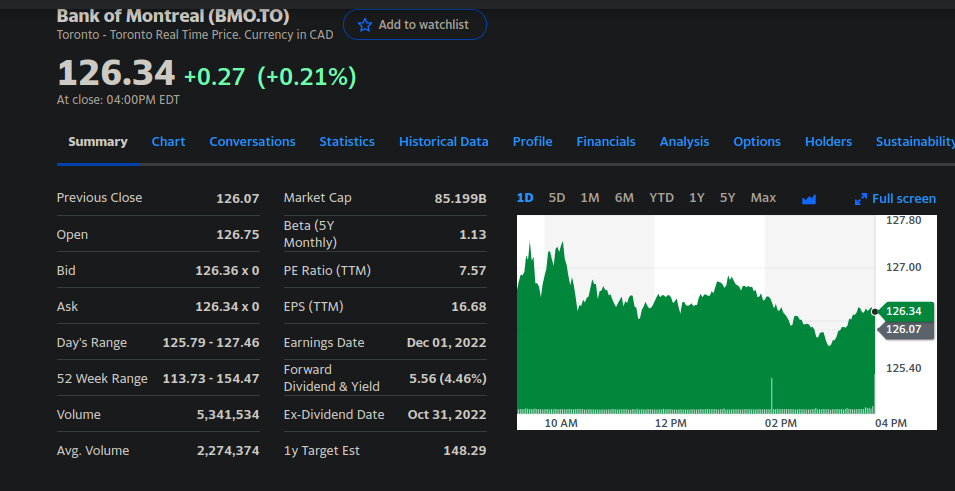
\includegraphics[width=\linewidth]{InvestingPics/figure1.png}
		\caption{View of \$BMO.TO in Yahoo Finance}
		\label{fig:chart1}
	\end{figure}

	%Figure \ref{fig:chart1} is a chart of BMO.TO

	\subsection{Analyzing the Summary Tab}

	\begin{itemize}
		\item {\bf Previous Close:} represents the last closing price reported of a security during a given time period; A security's previous close is an important value that is used by investors to chart gap patterns which can show substantial changes from a previous close to a new open.
		\item {\bf Open:} AKA the opening price; this is the value that a security is initially valued when the exchange opens for the day.
		\item {\bf Bid:} AKA the bidding price; A bid is an offer made by an investor, trader, or dealer in an effort to buy an asset or compete for a contract; The spread between the bid and asking price is a reliable indicator of supply \& demand for the security.
		\item {\bf Ask:} AKA asking price; The price at which someone is willing to sell a security for.
		\item {\bf Range:} Refers to the difference between the highest \& lowest prices a security or index ranges over an interval of time.
		\item {\bf Volume:} Trading volume is a measure of how much a given asset has been traded over a period of time. For stocks, volume is measured in the number of shares traded, for futures \& options, volume is based on how many contracts have changed hands. Volume can indicate market strength, as rising markets on increasing volume are typically viewed as strong and healthy.
		\item {\bf Avg. Volume:}
		\item {\bf Market Cap:} Market capitalization is calculated by multiplying the number of shares outstanding by the current price of a single share (i.e. A company with 50 mil shares \& a stock price \$100 per share would have a market cap of \$5 bil). Market cap is a metric based on stock price. \underline{Market capitalization is used to help define the value of a company when analyzing potential trade opportunities}. 
	\end{itemize}

\end{document}
